\documentclass{beamer}

 
\graphicspath{ {img/} }
\usepackage[utf8]{inputenc}
 
 
\title{Scala: The Hidden Gem of the JVM}
\author{Max Bo}
\institute{UQCS}
\date{2018}
 
 
 
\begin{document}
 
\frame{\titlepage}
 
\begin{frame}
% \frametitle{Sample frame title}

``2003 - A drunken Martin Odersky sees a Reese's Peanut Butter Cup ad featuring somebody's peanut butter getting on somebody else's chocolate and has an idea. He creates Scala, a language that unifies constructs from both object oriented and functional languages. This pisses off both groups and each promptly declares jihad."

    \textit{James Iry from `A Brief, Incomplete, and Mostly Wrong History of Programming Languages'}
\end{frame}

\begin{frame}
\frametitle{About Me}

\begin{itemize}
    \item 3rd year Computer Science @ UQ
    \item Currently interning at Skedulo
    \item @mb on the UQCS Slack
\end{itemize}

\end{frame}

\begin{frame}
    Why you should care
\end{frame}

\begin{frame}
    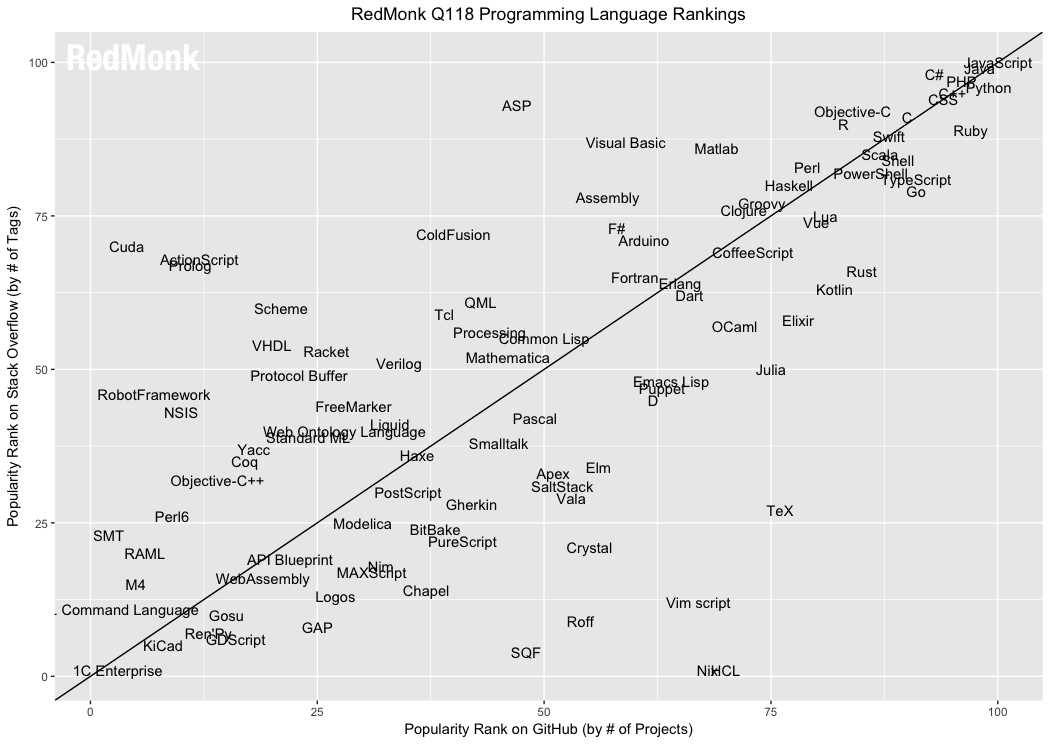
\includegraphics[width=\textwidth]{RedMonk.png}
    The RedMonk Programming Language Rankings: January 2018
\end{frame}

\begin{frame}
    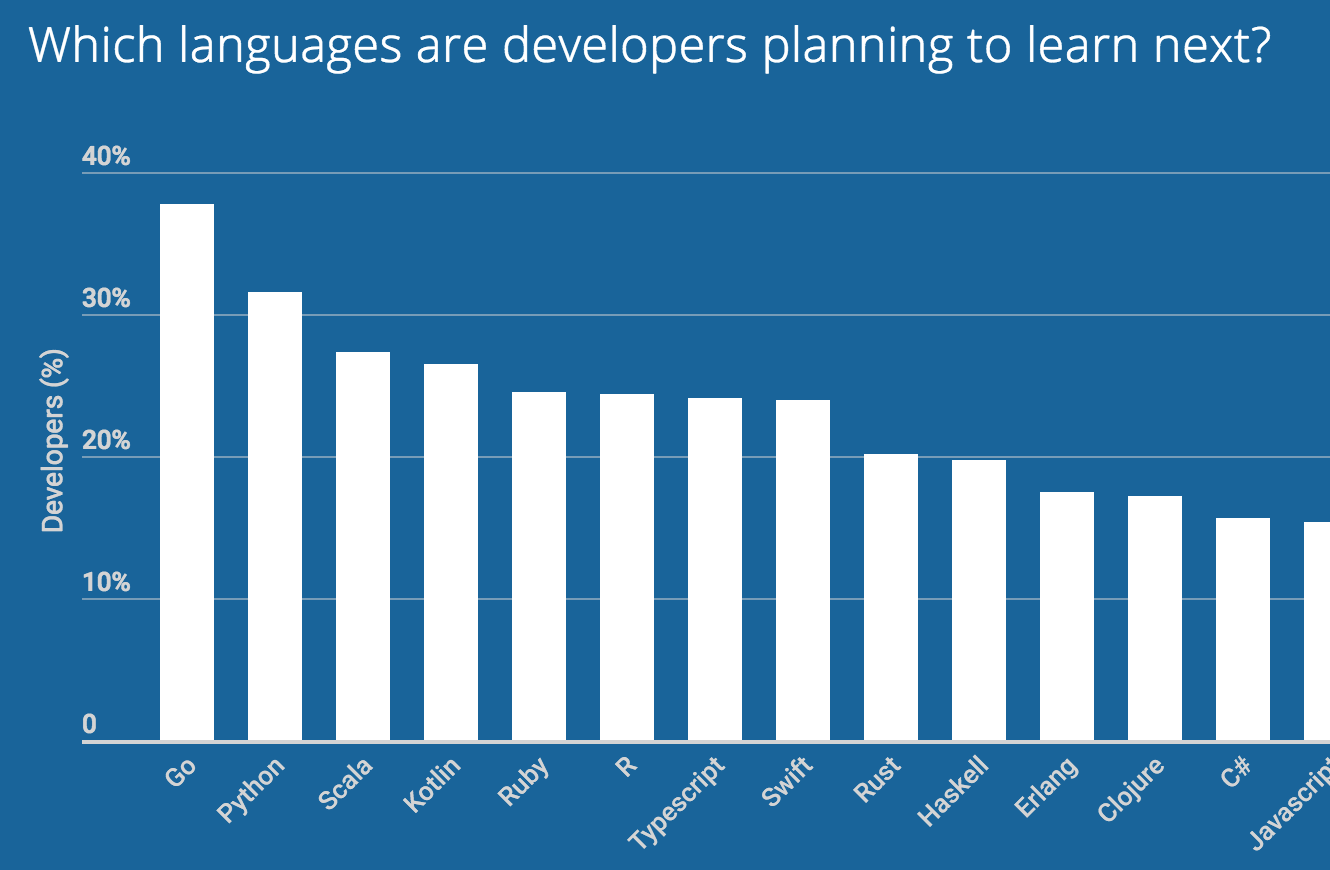
\includegraphics[width=\textwidth]{HackerRank.png}
    HackerRank 2018 Developer Skills Report
\end{frame}

\begin{frame}
    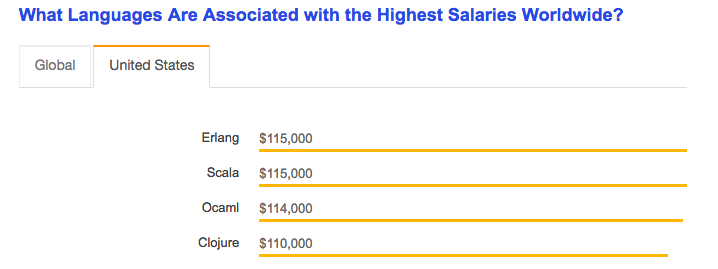
\includegraphics[width=\textwidth]{SO2018US.png}
\end{frame}

\begin{frame}
    
\includegraphics[width=\textwidth]{Platforms.png}
\end{frame}

\begin{frame}
    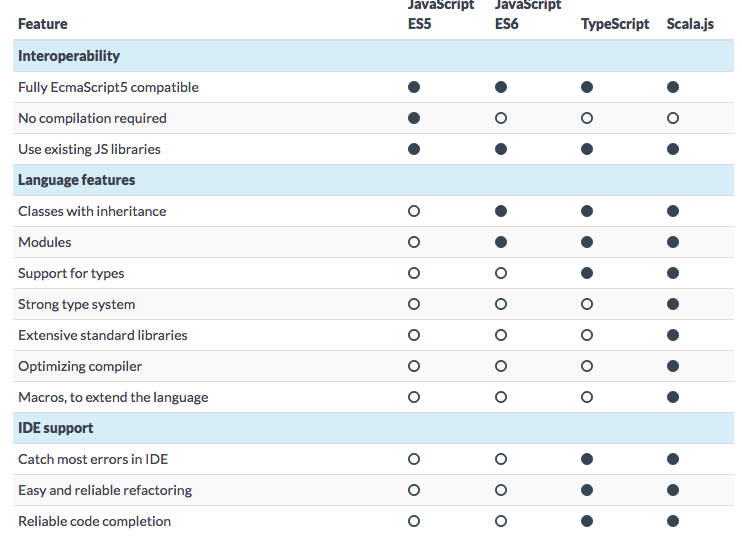
\includegraphics[width=\textwidth]{ScalaJS.png}
\end{frame}

\begin{frame}
    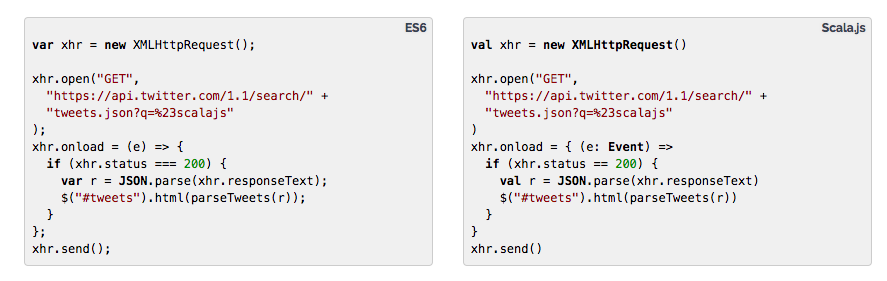
\includegraphics[width=\textwidth]{Interop.png}
\end{frame}

\begin{frame}
    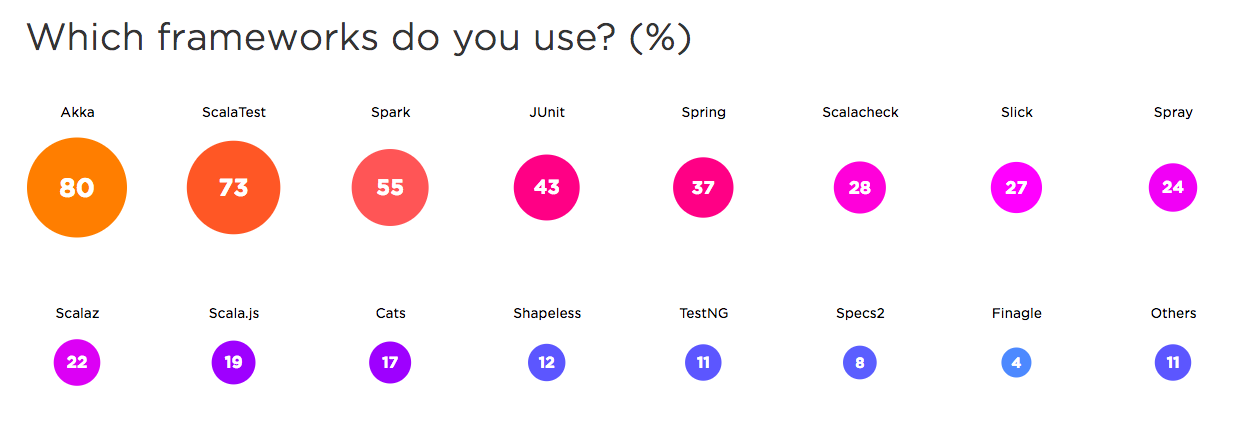
\includegraphics[width=\textwidth]{JetbrainsFrameworks.png}
\end{frame}


\end{document}
